% Created 2022-10-24 Mon 19:34
% Intended LaTeX compiler: pdflatex
\documentclass[a4paper,11pt,twoside]{article}
\usepackage[utf8]{inputenc}
\usepackage[T1]{fontenc}
\usepackage{graphicx}
\usepackage{longtable}
\usepackage{wrapfig}
\usepackage{rotating}
\usepackage[normalem]{ulem}
\usepackage{amsmath}
\usepackage{amssymb}
\usepackage{capt-of}
\usepackage{hyperref}
\usepackage{minted}
\usepackage{booktabs}
\usepackage{xcolor}
\usepackage{colortbl}
\usepackage{siunitx}
\usepackage{tabu}
\usepackage{etoolbox}
\usepackage{pdflscape}
\usepackage{pgfplots}
\usepackage{tikz}
\usepackage{nopageno}
\usepackage{amssymb}
\usepackage[margin=0.5in]{geometry}
\author{Adityan S}
\date{}
\title{Group Project}
\hypersetup{
 pdfauthor={Adityan S},
 pdftitle={Group Project},
 pdfkeywords={},
 pdfsubject={},
 pdfcreator={Emacs 28.2 (Org mode 9.6)}, 
 pdflang={English}}
\usepackage{biblatex}

\begin{document}

\maketitle
\tableofcontents

\clearpage

\section{Oscillation}
\label{sec:org8ab8d5c}
Consider the one-dimensional motion of a particle of mass \(m\) in a time independent potential \(V(x)\).Since the energy \(E\) is conserved, one can integrate the equation of motion and obtain a solution in a closed form.

$$
t-C = \sqrt{\frac{m}{2}}\int_{x_i}^x \frac{dx}{\sqrt{E-V(x)}}
$$

For the choice \(C=0\) , the particle is at the position \(x_i\) at the time \(t = 0\) and \(x\) refers to its position at any arbitrary time \(t\). Consider a particular case where the particle is in bound motion between twopoints \(a\) and \(b\) where \(V(x) = E\) for \(x = a, b\) and \(V(x) < E\) for \(a < x < b\). The time period of theoscillation \(T\) is given by,

$$
T = 2 \sqrt{\frac{m}{2}}\int_a^b \frac{dx}{\sqrt{E-V(x)}}
$$

\begin{center}
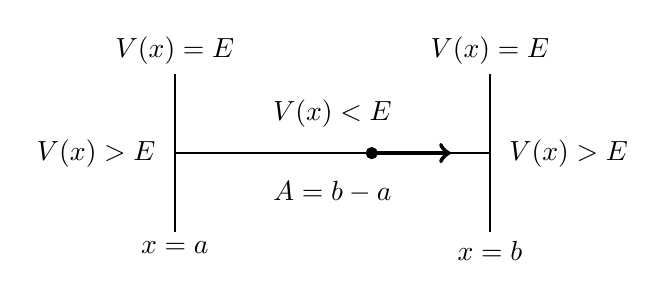
\begin{tikzpicture}
\draw[thick] (-2,0) -- (2,0);
\draw[thick] (-2,-1) -- (-2,1);
\draw[thick] (2,-1) -- (2,1);
\draw (2,-1) node [anchor=north]{$x=b$};
\draw (-2,-1) node [anchor=north]{$x=a$};
\draw (0,0.5) node {$V(x)<E$};
\draw (-3,0) node {$V(x)>E$};
\draw (3,0) node {$V(x)>E$};
\draw (2,1) node [anchor=south]{$V(x)=E$};
\draw (-2,1) node [anchor=south]{$V(x)=E$};
\draw (0,-0.5) node {$A=b-a$};
\filldraw [black] (0.5,0) circle (2pt);
\draw[ultra thick, ->] (0.5,0) -- (1.5,0);
\end{tikzpicture}
\end{center}

\subsection{First consider a particle with \(m = 1 kg\) in the potential \(V_1(x) = 0.5 \alpha x^2\) with \(\alpha =4 kg sec^2\). Numerically calculate the time period of oscillation and check this against the expected value. Verify that the frequency does not depend on the amplitude of oscillation.}
\label{sec:org67e05d3}


\begin{center}
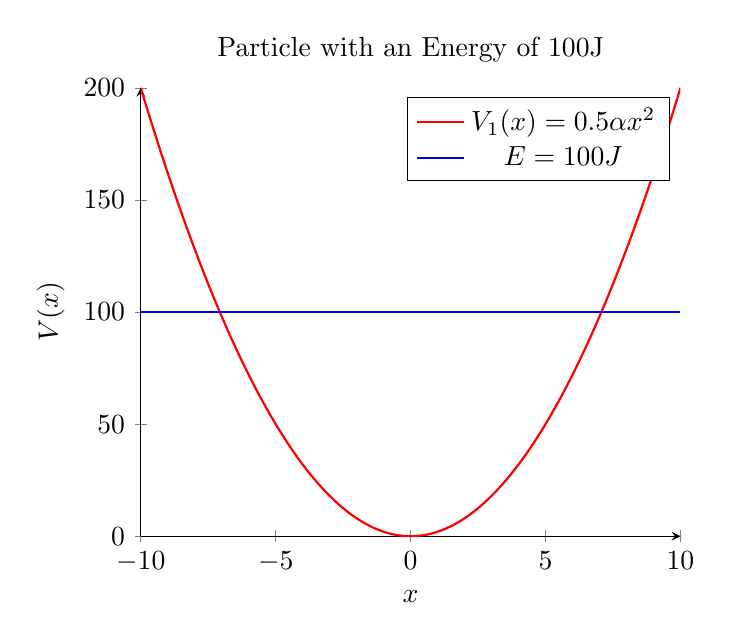
\begin{tikzpicture}
\begin{axis}[title={Particle with an Energy of 100J}, axis lines=left, xlabel=$x$, ylabel=$V(x)$]
\addplot[domain=-10:10, samples=200, thick, red] {2*x^2};
\addlegendentry{$V_1(x)=0.5\alpha x^2$};
\addplot[domain=-10:10, samples=200, thick, blue] {100};
\addlegendentry{$E = 100J$};
\end{axis}
\end{tikzpicture}
\end{center}

From the above plot, we infer that the for a value of Energy \(E\), the particle is bound for specific values of \(a\) and \(b\) (decided by \(E\)).

$$
E = V_1(a)=V_1(b) = 2x^2
$$

$$
 \implies a = - \sqrt{\frac{E}{2}} = -A, \quad b = +\sqrt{\frac{E}{2}} = +A
$$

Hence Amplitude of oscillation is a function of Energy.

$$
A(E) = b-a = \sqrt{\frac{E}{2}} \implies E = 2A^2
$$


\clearpage

From the above equations, the analytic solution,


$$
T = \frac{1}{A}\int_{-A}^{+A} \frac{dx}{\sqrt{1-(\frac{x}{A})^2}} = sin^{-1}{\Big(\frac{x}{A}\Big)} \Big|_{-A}^{ +A} = \pi \quad (sec)
$$

Using integral identities,  \(T\) can be written as,

$$
T = \int_{-1}^{+1} \frac{dx}{\sqrt{1-x^2}}
$$

Let us solve the above numerically,

\begin{minted}[breaklines=true,breakanywhere=true]{f90}
program occilation1
  use mods
  implicit none
  integer :: i
  integer, parameter :: N = 2
  real(dp), dimension(N) :: x, w
  call gauss_chebyshev_1(x, w)
  print *, sum(w)
end program occilation1
\end{minted}


\begin{minted}[breaklines=true,breakanywhere=true]{sh}
fpm run oscillation1
\end{minted}

\begin{verbatim}
3.141592653589793
\end{verbatim}


The above integral \(T = 3.141592653589793 \approx \pi \neq T(E,A)\) . Hence the timeperiod is independent of Amplitude.


\subsection{Next consider a potential \(V_2(x) = e^{0.5αx^2 } -1\). Numerically verify that for small amplitude oscillations you recover the same results as the simple harmonic oscillator.}
\label{sec:org93ec037}

\begin{center}
\begin{tikzpicture}
\begin{axis}[title={Particle with an Energy of 0.5J}, axis lines=left, xlabel=$x$, ylabel=$V(x)$]
\addplot[domain=-1:1, samples=200, thick, green] {2*x^2};
\addlegendentry{$V_1(x)=0.5\alpha x^2$};
\addplot[domain=-1:1, samples=200, thick, red] {e^(2*x^2) -1};
\addlegendentry{$V_2(x) = e^{0.5αx^2 } -1$};
\addplot[domain=-1:1, samples=200, thick, blue] {0.5};
\addlegendentry{$E = 0.5J$};
\end{axis}
\end{tikzpicture}
\end{center}

From the above plot, we can infer that for particles of very small energies the given potential behaves as the simple harmonic occilator.

Let us verify the above statement numerically,

$$
T =\frac{\sqrt2}{e^{A^2}} \int _{-A}^{A} \frac{dx}{\sqrt{1-e^{2(x^2-A^2)}}} = \frac{\sqrt2A}{e^{A^2}} \int _{-1}^{1} \frac{dx}{\sqrt{1-e^{2A^2(x^2-1)}}}
$$

$$
\implies A = \pm \sqrt{\frac{\ln{(E+1)}}{2}}
$$

\clearpage

\begin{minted}[breaklines=true,breakanywhere=true]{f90}
program occilation2
  use mods
  implicit none
  integer :: i
  integer, parameter :: N = 5000
  real(dp), dimension(100) :: A
  real(dp), dimension(N) :: x, w
  call gauss_legendre(x, w)
  call linspace(0.01_dp, 1.0_dp, A)
  open(1, file='./src/oscillation/o2T.csv', status='old')
  do i=1,100
     write (1,'(1f10.7, a, 1f10.7)') A(i), " ", sum((sqrt(2._dp)*A(i)/(e**(A(i)**2)))*w*(1/sqrt(1-e**(2*(A(i)**2)*((x**2)-1)))))
  end do
  write (*, *) "$A$ $T$"
  do i=1,10
     write (*,'(1f10.7, a, 1f10.7)') A(i), " ", sum((sqrt(2._dp)*A(i)/(e**(A(i)**2)))*w*(1/sqrt(1-e**(2*(A(i)**2)*((x**2)-1)))))
  end do
end program occilation2
\end{minted}


\begin{minted}[breaklines=true,breakanywhere=true]{sh}
fpm run oscillation2
\end{minted}

\begin{center}
\begin{tabular}{rr}
\hline
\(A\) & \(T\)\\\empty
\hline
0.01 & 3.1410088\\\empty
0.02 & 3.1403022\\\empty
0.03 & 3.1391248\\\empty
0.04 & 3.1374772\\\empty
0.05 & 3.13536\\\empty
0.06 & 3.1327742\\\empty
0.07 & 3.1297208\\\empty
0.08 & 3.1262011\\\empty
0.09 & 3.1222167\\\empty
0.1 & 3.1177692\\\empty
\hline
\end{tabular}
\end{center}


\begin{center}
\begin{tikzpicture}
\begin{axis}[title={Amplitude vs Timeperiod} , axis lines=left, xlabel=$A$, ylabel=$T(A)$]
\addplot[mark=none,thick,red] table {./src/oscillation/o2T.csv};
\addlegendentry{$T(V_2)$};
\addplot[domain=0:1, samples=200, thick, blue] {3.14};
\addlegendentry{$T(V_1)$};
\end{axis}
\end{tikzpicture}
\end{center}


Hence for Oscillation of small amplitudes, we get the same results as simple harmonic oscillator.

\clearpage

\section{Black Body Spectrum}
\label{sec:orgd6d43ce}
Quantum mechanics began with Planck’s fit to the spectrum of black body radiation:

$$
I(\nu , T) = \frac{2h\nu^3}{c^2} \frac{1}{e^{\frac{h\nu}{kT}}-1}
$$

Here \(I(\nu,T)\) is the energy per unit time of radiation with frequency \(\nu\) emitted per unit area of emitting surface, per unit solid angle, and per unit frequency by a black body at temperature \(T\). The parameter \(h\) is Planck’s constant, \(c\) is the speed of light in vacuum, and \(k\) is Boltzmann constant. The Cosmic Background Explorer (COBE) project measured the cosmic background radiation and obtained the results given in the file \texttt{cobe.dat}

\begin{minted}[breaklines=true,breakanywhere=true]{sh}
cat ./src/cobe/cobe.dat
\end{minted}

\begin{center}
\begin{tabular}{rrr}
\hline
\(\widetilde{\nu}\) & \(I(\nu ,T)\) & Error\\\empty
\hline
2.27 & 200.723 & 14\\\empty
2.72 & 249.508 & 19\\\empty
3.18 & 293.024 & 25\\\empty
3.63 & 327.77 & 23\\\empty
\ldots{} & \ldots{} & \ldots{}\\\empty
20.42 & 7.087 & 88\\\empty
20.87 & 5.801 & 155\\\empty
21.33 & 4.523 & 282\\\empty
\hline
\end{tabular}
\end{center}

\subsection{Plot the COBE data and see if it has a shape similar to the black body spectrum first explained by Planck.}
\label{sec:org23973c9}


\begin{center}
\begin{tikzpicture}
\begin{axis}[title={COBE Measurement} , axis lines=left, xlabel=$\widetilde{\nu}$, ylabel=$I$]
\addplot[only marks,mark=halfcircle,blue] table {./src/cobe/cobeplot.csv};
\addplot[] coordinates{(0,0)(25,0)};
\end{axis}
\end{tikzpicture}
\end{center}

Yes, the given data has a shape similar to the black body spectrum first explained by Planck.



\subsection{Use these data to deduce the temperature T of the cosmic microwave background radiation.}
\label{sec:org2584fd2}
$$
I =  \frac{0.0014745 \nu^3}{e^{b\nu}-1} \quad in \quad \frac{MJy}{sr}
$$

$$
\nu = 30\widetilde{\nu}  \quad in \quad GHz, \quad
\widetilde{\nu} \quad in \quad \frac{1}{cm^{-1}}
$$
$$
T = 10^9 \frac{h}{bk}, \quad b \quad in \frac{1}{GHz}, \quad T \quad in \quad K
$$


\clearpage

Using Least Square Optimization

$$
b = min\{ \sum_{i=1}^{43} r_i(b) \} = min\{ \sum_{i=1}^{43} ( \frac{0.0014745 \nu_i^3}{e^{b\nu_i}-1} - I_i)^2 \}
$$

Let the Initial Guess for \(b\) be
\(b = 0.048  \implies T \approx 1K\)

\begin{minted}[breaklines=true,breakanywhere=true]{python}
import numpy as np
from scipy.optimize import least_squares
import pandas as pd
import warnings
warnings.filterwarnings("ignore")

data = pd.read_csv("src/cobe/cobeplot.csv", header=None, delim_whitespace=True)
vbi = np.asarray(data[0])
Ii = np.asarray(data[1])
vi = 30 * vbi

def r(b, vi, Ii):
    return ((0.0014745*pow(vi,3))/(np.exp(b*vi)-1) - Ii)**2

b = least_squares(r, 0.048, args=(vi, Ii))
print(b.x)
\end{minted}

\begin{verbatim}
[0.01760962]
\end{verbatim}


$$
b = 0.01760962  \implies T \approx 2.73K
$$


\subsection{Assess the accuracy of the fit by doing a Pearson's \(\chi^2\) (chi-squared) analysis.}
\label{sec:org3d68c8f}


\begin{minted}[breaklines=true,breakanywhere=true]{f90}
program cobe
  use mods
  implicit none

  real(dp) :: v(200), I(200), vi(43), vbi(43), Ii(43), erri(43), chisq
  integer :: m, j

  m = 43 ! No of data points
  open(99, file="./src/cobe/cobe.dat")
  open(98, file="./src/cobe/cobefit.csv")
  open(97, file="./src/cobe/cobeplotfreq.csv")

  do j=1, m
     read(99, *) vbi(j), Ii(j), erri(j)
  end do
  vi = 30._dp*vbi
  do j=1, m
     write(97, *) vi(j), Ii(j)
  end do
  call linspace(0._dp, 1000._dp, v)
  do j=1, 200
     I(j) = blackbody(v(j))
     write(98, "(2f20.14)") v(j), I(j)
  end do

  chisq = 0._dp
  do j=1,m
     chisq = chisq + (((Ii(j) - blackbody(vi(j)))**2._dp)/(blackbody(vi(j))))
  end do
  write(*, "(1f20.14)") chisq
  
  close(99)
  close(98)
  close(97)
contains
  real(dp) function blackbody(v) result(I)
    real(dp), intent(in) :: v
    I = (0.0014745_dp*(v**3._dp))/(exp(v*0.01760962_dp)-1._dp)
  end function blackbody
end program cobe
\end{minted}

\begin{center}
\begin{tikzpicture}
\begin{axis}[title={COBE Fit} , axis lines=left, xlabel=$\nu(GHz)$, ylabel=$I(MJy/sr)$]
\addplot[only marks,mark=halfcircle,blue] table {./src/cobe/cobeplotfreq.csv};
\addplot[mark=none,red,thick] table {./src/cobe/cobefit.csv};
\end{axis}
\end{tikzpicture}
\end{center}


\begin{center}
\begin{tabular}{ll}
\hline
Hypothesis & Plank's Law Fit\\\empty
Expected Values & \(I(\nu_i)\)\\\empty
Observes Values & \(I_i\)\\\empty
No of Observations & 43\\\empty
\hline
\end{tabular}
\end{center}

$$
\chi^2 = \sum_{i=1}^{43} \frac{(I_i - I(\nu_i))^2}{I(\nu_i)}
$$

\begin{minted}[breaklines=true,breakanywhere=true]{sh}
fpm run cobe
\end{minted}

\begin{verbatim}
0.04425666834533
\end{verbatim}


$$
\chi^2 = 0.04425666834533 < 1
$$

Hence it is a good fit

\clearpage

\section{Modules}
\label{sec:orgcfecace}

\subsection{Module \texttt{mods} consists of all subroutines, variables and procedures that are used in this report. The codeblocks below are all part of the file \texttt{mods.f90}}
\label{sec:orgbacc95e}

\begin{minted}[breaklines=true,breakanywhere=true]{f90}
module mods
  use, intrinsic :: iso_fortran_env, only: dp => real64
  use stdlib_quadrature, only: gauss_legendre
  implicit none

  real(dp), parameter :: pi=3.14159265358979323846_dp
  real(dp), parameter :: e= 2.7182818284590452353_dp

\end{minted}
\subsection{Interfaces}
\label{sec:orgd758085}

\begin{minted}[breaklines=true,breakanywhere=true]{f90}
contains
\end{minted}
\subsection{Routines for Array Manipulation}
\label{sec:orgdc7da08}
\subsubsection{Linspace Subroutine for creating an array(sequence) with the equal step value.}
\label{sec:org5426f0b}

\begin{minted}[breaklines=true,breakanywhere=true]{f90}
subroutine linspace(from, to, array)
  real(dp), intent(in) :: from, to
  real(dp), intent(out) :: array(:)
  real(dp) :: range
  integer :: n, i
  n = size(array)
  range = to - from
  if (n == 0) return
  if (n == 1) then
     array(1) = from
     return
  end if
  do i=1, n
     array(i) = from + range * (i - 1) / (n - 1)
  end do
end subroutine linspace
\end{minted}

\subsection{Routines for Numerical Integration}
\label{sec:orgac11445}
\subsubsection{N-point Gauss Chebyshev Quadrature of 1st kind.}
\label{sec:orgba43c3a}

$$
\int _{-1}^{+1}{\frac {f(x)}{\sqrt {1-x^{2}}}}\,dx\approx \sum _{i=1}^{n}w_{i}f(x_{i})}
$$

$$
x_{i}= \cos \left({\frac {2i-1}{2n}}\pi \right) \quad w_{i}={\frac {\pi }{n}}
$$

\begin{minted}[breaklines=true,breakanywhere=true]{f90}
subroutine gauss_chebyshev_1(x, w)
  real(dp), intent(out) :: w(:), x(:)
  integer :: n, i
  n = size(w)
  do i=1, n
     x(i) = cos((pi*(2*real(i)-1))/(2*real(n)))
     w(i) = pi/real(n)
  end do
end subroutine gauss_chebyshev_1
\end{minted}

\subsubsection{N-point Gauss Legendre Quadrature of 1st kind.}
\label{sec:org0997182}

$$
\int _{-1}^{+1}{f(x)}\,dx\approx \sum _{i=1}^{n}w_{i}f(x_{i})}
$$

$$
w_{i}=\frac {2}{\left(1-x_{i}^{2}\right)\left[P'_{n}(x_{i})\right]^{2}} \quad   P_n(x_i)=0
$$

\begin{minted}[breaklines=true,breakanywhere=true]{f90}
!use stdlib_quadrature, only: gauss_legendre
\end{minted}

\subsection{Routines for Optimization of Non Linear Equation}
\label{sec:orgdcc875c}
Using SCIPY
\subsection{End of module \texttt{mods}}
\label{sec:org5383ca6}

\begin{minted}[breaklines=true,breakanywhere=true]{f90}
end module mods
\end{minted}


\clearpage
\end{document}